% This is "sig-alternate.tex" V2.0 May 2012
% This file should be compiled with V2.5 of "sig-alternate.cls" May 2012
%
% This example file demonstrates the use of the 'sig-alternate.cls'
% V2.5 LaTeX2e document class file. It is for those submitting
% articles to ACM Conference Proceedings WHO DO NOT WISH TO
% STRICTLY ADHERE TO THE SIGS (PUBS-BOARD-ENDORSED) STYLE.
% The 'sig-alternate.cls' file will produce a similar-looking,
% albeit, 'tighter' paper resulting in, invariably, fewer pages.
%
% ----------------------------------------------------------------------------------------------------------------
% This .tex file (and associated .cls V2.5) produces:
% 1) The Permission Statement
% 2) The Conference (location) Info information
% 3) The Copyright Line with ACM data
% 4) NO page numbers
%
% as against the acm_proc_article-sp.cls file which
% DOES NOT produce 1) thru' 3) above.
%
% Using 'sig-alternate.cls' you have control, however, from within
% the source .tex file, over both the CopyrightYear
% (defaulted to 200X) and the ACM Copyright Data
% (defaulted to X-XXXXX-XX-X/XX/XX).
% e.g.
% \CopyrightYear{2007} will cause 2007 to appear in the copyright line.
% \crdata{0-12345-67-8/90/12} will cause 0-12345-67-8/90/12 to appear in the copyright line.
%
% ---------------------------------------------------------------------------------------------------------------
% This .tex source is an example which *does* use
% the .bib file (from which the .bbl file % is produced).
% REMEMBER HOWEVER: After having produced the .bbl file,
% and prior to final submission, you *NEED* to 'insert'
% your .bbl file into your source .tex file so as to provide
% ONE 'self-contained' source file.
%
% ================= IF YOU HAVE QUESTIONS =======================
% Questions regarding the SIGS styles, SIGS policies and
% procedures, Conferences etc. should be sent to
% Adrienne Griscti (griscti@acm.org)
%
% Technical questions _only_ to
% Gerald Murray (murray@hq.acm.org)
% ===============================================================
%
% For tracking purposes - this is V2.0 - May 2012

\documentclass{sig-alternate-2013}

\usepackage{url} 
\usepackage{color}
\usepackage[utf8]{inputenc}
\usepackage{graphicx}
\usepackage{booktabs}
\usepackage{array}
\usepackage{amsfonts}
%\usepackage{amsthm}
\usepackage{tikz}
\usepackage{amsmath}
\usepackage{float}
\usepackage{graphicx}
\usepackage{caption}
\DeclareCaptionType{copyrightbox}
\usepackage{subcaption}
\usepackage{color}
\usepackage{amssymb}
\usepackage{bm}
\usepackage{calc}

\usepackage{fancyhdr} % This should be set AFTER setting up the page geometry
\pagestyle{fancy} % options: empty , plain , fancy
\renewcommand{\headrulewidth}{0pt} % customise the layout...
\lhead{}\chead{}\rhead{}
\lfoot{}\cfoot{\thepage}\rfoot{}

\newtheorem{theorem}{Theorem} 
\newtheorem{lemma}{Lemma}
\newtheorem{propn}{Proposition}
%\newtheorem*{thmm}{Theorem}
\newtheorem{remk}{Remark} 
\newtheorem{corol}{Corollary}
\newtheorem{definition}{Definition}



\newtheorem{thm}{Theorem}[section] 
\newtheorem{prop}[thm]{Proposition} 
\newtheorem{lem}[thm]{Lemma}
\newtheorem{cor}[thm]{Corollary} 
\newtheorem{con}[thm]{Conjecture} 

%\theoremstyle{definition}
\newtheorem{defn}[thm]{Definition}
%\newtheorem*{rem}{Remark}
%\newtheorem*{nota}{Notation}
%\newtheorem*{nota}{Notation}
\newtheorem{cla}[thm]{Claim}
\newtheorem{ex}[thm]{Example}
\newtheorem{exs}[thm]{Examples}
%\newtheorem*{exer}{Exercise}
\newtheorem{case}{Case}
\newtheorem{conj}{Conjecture}

\definecolor{sotonblue}{rgb}{0.0,0.394,0.597}

\newcommand{\pspace}{$(\Omega_\alpha,\mathcal{F}_\alpha,P_\alpha)$ } 
\DeclareMathOperator{\Aut}{Aut}
\DeclareMathOperator{\Pspace}{(\Omega, \mathcal{F},\mathbb{P})}
\DeclareMathOperator{\Pspacen}{(\Omega_n, \mathcal{F}_n,\mathbb{P}_n)}

\DeclareMathOperator{\X}{\mathcal{X}}
\DeclareMathOperator{\Y}{\mathcal{Y}}
\DeclareMathOperator{\A}{\mathcal{A}}
\DeclareMathOperator{\B}{\mathcal{B}}
\DeclareMathOperator{\F}{\mathcal{F}}
\newcommand*{\refname}{Bibliography}
\begin{document}
%
% --- Author Metadata here ---
\conferenceinfo{Workshop on the theory and practice of social machines @ WWW2014}{2014, Seoul, South Korea}
%\CopyrightYear{2007} % Allows default copyright year (20XX) to be over-ridden - IF NEED BE.
%\crdata{0-12345-67-8/90/01} % Allows default copyright data (0-89791-88-6/97/05) to be over-ridden - IF NEED BE.
% --- End of Author Metadata ---

\title{Community structure for efficient information flow in `ToS;DR', a social machine for parsing legalese}
%
% You need the command \numberofauthors to handle the 'placement
% and alignment' of the authors beneath the title.
%
% For aesthetic reasons, we recommend 'three authors at a time'
% i.e. three 'name/affiliation blocks' be placed beneath the title.
%
% NOTE: You are NOT restricted in how many 'rows' of
% "name/affiliations" may appear. We just ask that you restrict
% the number of 'columns' to three.
%
% Because of the available 'opening page real-estate'
% we ask you to refrain from putting more than six authors
% (two rows with three columns) beneath the article title.
% More than six makes the first-page appear very cluttered indeed.
%
% Use the \alignauthor commands to handle the names
% and affiliations for an 'aesthetic maximum' of six authors.
% Add names, affiliations, addresses for
% the seventh etc. author(s) as the argument for the
% \additionalauthors command.
% These 'additional authors' will be output/set for you
% without further effort on your part as the last section in
% the body of your article BEFORE References or any Appendices.

\numberofauthors{2} % in this sample file, there are a *total*
% of EIGHT authors. SIX appear on the 'first-page' (for formatting
% reasons) and the remaining two appear in the \additionalauthors section.
%
\author{
% You can go ahead and credit any number of authors here,
% e.g. one 'row of three' or two rows (consisting of one row of three
% and a second row of one, two or three).
%
% The command \alignauthor (no curly braces needed) should
% precede each author name, affiliation/snail-mail address and
% e-mail address. Additionally, tag each line of
% affiliation/address with \affaddr, and tag the
% e-mail address with \email.
%
% 1st. author
\alignauthor
Reuben Binns, David Matthews\\
       \affaddr{Web Science Doctoral Training Centre}\\
       \affaddr{University of Southampton}\\
       \affaddr{Southampton, UK}\\
       \email{\{rb5g11,dm1x07\}@soton.ac.uk}
}
% There's nothing stopping you putting the seventh, eighth, etc.
% author on the opening page (as the 'third row') but we ask,
% for aesthetic reasons that you place these 'additional authors'
% in the \additional authors block, viz.
%\additionalauthors{Additional authors: John Smith (The Th{\o}rv{\"a}ld Group,
%email: {\texttt{jsmith@affiliation.org}}) and Julius P.~Kumquat
%(The Kumquat Consortium, email: {\texttt{jpkumquat@consortium.net}}).}
%\date{30 July 1999}
% Just remember to make sure that the TOTAL number of authors
% is the number that will appear on the first page PLUS the
% number that will appear in the \additionalauthors section.

\maketitle
\begin{abstract}

This paper presents a case study of `Terms-of-Service; Didn't Read', a social machine to curate, parse, and rate website terms and privacy policies. We examine the relationships between its human contributors and machine counterparts to determine community structure and information flow.

\end{abstract}

% A category with the (minimum) three required fields
\category{H.1.2}{User/Machine Systems}{Human information processing}
\category{G.2.3}{Discrete Mathematics}{Applications}

\terms{Human Factors, Measurement, Theory}

\keywords{Social Machines; Terms of Service; Privacy; Legal Informatics; Network Science, Community structure}
\section{Introduction}

Social machines are new combinations of human and machine activity that engage in complex activities and solve problems which were previously difficult or costly for humans or machines to do alone \cite{shadbolt:classif}. An interesting application of social machines is to the curation, analysis and rating of legal documents and advice. Contracts, terms-of-service, privacy policies, and licenses all serve important functions in a range of online and offline interactions. However, they incur significant costs on interacting parties as they are often written in complex legalistic language (sometimes referred to as `legalese') which is time-consuming and difficult for individuals to understand without formal training. In addition, despite advances in automatic parsing techniques made in semantic processing and legal informatics \cite{franc:semantic, spinosa:nlp}, computational processes alone may be insufficient. Instead, social machines aimed at handling these tasks and functions are emerging. These systems aim to capture the activity of human actors who write, develop, read, modify, sign, or abide by such texts, and aggregate that activity to produce new content and services.

We used an existing classificatory framework for social machines to search for and identify systems in this area \cite{shadbolt:classif}. For the purposes of this paper, our broader analysis of the domain of social machines for parsing legalese has been discarded. We focus here on just one case study, the `Terms of Service; Didn't Read' project, a platform for analysing and rating website terms and privacy policies.

\section{Case study: ToS;DR}

The ToS;DR platform has around 500 users, who communicate primarily through an open mailing list. Its stated aim is to `fix the biggest lie on the internet' - namely, the statement that `I have read and agreed to the terms'. Participants identify, discuss, and annotate clauses in terms-of-service and privacy policies, rating them as either `good', `bad', or `neutral'. This activity generates the raw data which drives the service – as they explain it, `every thread on the mailing list is a data point'. The number of good, bad and neutral points are tallied to produce an overall rating of a policy. The ratings serve data via an API to other services including a browser plugin.

In order to keep track of changing policies, an automated web crawler called ToSBACK regularly crawls an index of websites and notifies the human participants of any changes to the policies which may need to be reviewed. Any participant can add a website to the index, which is a list of XPath addresses.

The ToS;DR platform provides a case study of how legalese text can be parsed through a social machine. The system receives an input of `raw legalese', analyses its parts in terms of `good' and `bad', and outputs an overall score. An interesting aspect of this process is the community structure and the way information flows within it. In order to explore this we used the Girvan and Newman (GN) algorithm for identifying communities in complex networks \cite{gnm:comm}. We ran the same analysis on the data before and after the introduction of the ToSBACK crawler, in order to test how the introduction of a computational actor affected community structure.

\subsection{Method}

We built two graphs $G_{1}$ and $G_2$ corresponding to the mailing list archive before and after the ToSBack bot began contributing. The vertex sets of both graphs are made up of all the regularly interacting contributors to the mailing list. In total, 2,345 interactions were analysed, from between 28-35 active users. An edge was placed between two vertices if the relevant contributors responded, or were responded to by another contributor. These edges were then weighted by the number of interactions between the relevant contributors. Finally we applied the GN algorithm to both graphs. GN detects bottlenecks in the graph of social interactions and splits the graph along these bottlenecks into  a nested hierarchy of communities [See appendix \ref{Girvan and Newman Algorithm}].

\subsection{Results}
Tree $T_1$ (Figure \ref{fig:t1}) was built via the GN algorithm from the mailing list \emph{prior} to the introduction of the ToSBack bot, and corresponds to a nested hierarchy of communities. The vertex labelled 1 represents the entire mailing list and every interaction between contributors, whereas the vertices 2 and 17 represent sub-communities that we will call $C2$ and $C17$ respectively. Since 2 is adjacent to 3 and 4 there also exist sub-communities of $C2$ that we denote $C3$ and $C4$. One can deduce from the GN algorithm that leaf vertices of $T_1$ correspond to a single contributor, thus $C3$ is a community of precisely 1 person. On the other hand $C4$ indicates a much larger community – ($C2$ without one contributor).

In general a subtree of the tree associated to a network using the GN algorithm that is “close ” to a line indicates a hub and spoke community. We have highlighted four line-like subtrees in $T_1$; these subtrees can be recognised as the areas of discussion initiated by or frequently involving particular members.

We can formalise the notion of “line-like” subtrees by analysing the \emph{symmetry} of  
a tree.  One can measure how symmetric
a tree is by calculating the number of permutations, $\lvert \Aut(T) \rvert$, of the
vertices (of that graph) that preserve adjacent vertices \cite{bela:mgt}. We
call the set of such permutations the automorphism group of $T$. In general a low $\lvert \Aut(T) \rvert$ coincides with the presence of one or several long line-like subtrees.  We calculated that $\lvert \Aut(T_1)\rvert = 16$ and $\vert \Aut(T_2)\rvert = 24$.  This shows a marked
increase in the cardinality of the automorphism group and
therefore increased symmetry which is further entrenched by normalisation of $\Aut(T)$.
\begin{figure}[H]
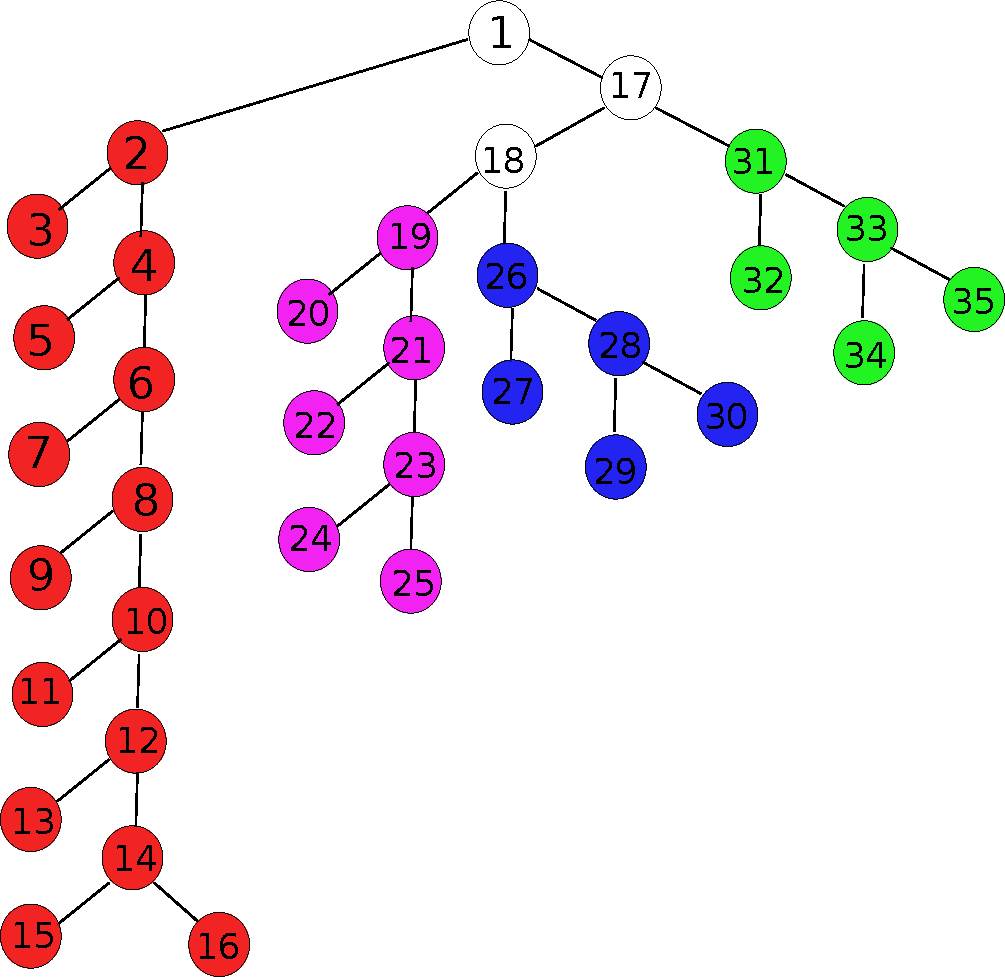
\includegraphics[width=7.5cm, height  = 5cm]{t15.pdf}\caption{ The tree, $T_1$, built via the GN algorithm that corresponds to the mailing list \emph{prior} to the ToSBack bot contributions.}\label{fig:t1}
\end{figure}
\begin{figure}[H]
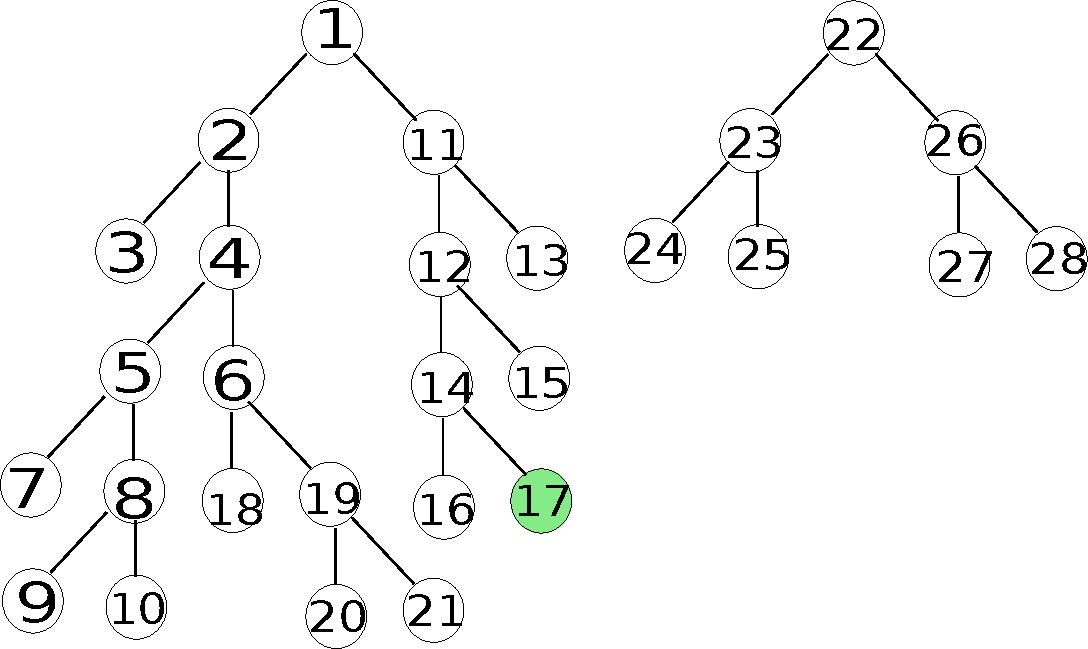
\includegraphics[width=7.5cm, height=3.5cm]{t26.pdf}\caption[width=7]{ The tree, $T_2$, built via the GN algorithm that corresponds to the mailing list \emph{after} the ToSBack bot contributions began.  Vertex 17 [green] indicates the bot. }\label{fig:t2}
\end{figure}

\subsection{Discussion}
We see two distinct community structures before and after the introduction of the ToSBack bot. Notice the asymmetry of the very long branch (red in $T_1$), which represents one particular user's tendency to interact with a disproportionate number of contributors. In contrast, after the introduction of the bot, the network is more balanced with no one information hub. %The first graph consists of one connected tree while the other is two largely separate trees, indicating two separated communities.

One explanation for the new structure is suggested by research into how natural structures become optimised. Self-similarity in natural structures like rivers ensures that these structures develop in an optimal way \cite{murray:min}. Guimera \emph{et. al.} show that this principle is also true for communities; they tend to self-organise to form an optimal structure \cite{guimera:comm}. One way of measuring self-similarity in a graph is to find the order of the symmetry group or group of automorphisms of that graph. The increased symmetry in $T_2$ may therefore be a result of self-organisation that occurred after the introduction of TosBack, allowing for more efficient dissemination of information.

Finally, one particular user began interacting heavily with the bot, accounting for the overwhelming majority of interactions with the bot (86\%). During this period, the user's importance in the network grew, triggering more responses than in the previous period (while her total contributions remained stable). A possible explanation for this is that this user became a filter between the new content generated by the bot and other (human) participants.

\section{Conclusion}

%Reflecting on ToS;DR in depth raises some interesting points of connection with previous work on the theory of social machines. First, as proposed in previous work, social machines should be regarded as `networks of networks' \cite{tinati:htp}, and similarly, as `nested' within each other at different levels of a `polyarchy' \cite{shadbolt:classif}. Our examination of Tos;DR lends weight to both perspectives; our analysis reveals distinct networks of contributors within the larger network, which is itself, in part, nested within the even larger Google Groups network.

%Second, ToS;DR and ToSBACK are examples of two pre-existing social machines (both of which consisted of human and machine actors), which became appropriated by each other and amalgamated into a new composite social machine (illustrating at least two distinct `phases' of development \cite{tinati:htp}). In addition, the websites that this composite social machine interacts with (through scraping, annotating and rating), are often themselves instances of social machines (i.e. Facebook or Wikipedia). This emphasises the importance of recognising the extent to which social machines interact with each other in complex ways which might otherwise be overlooked if considered individually \cite{deroure:obs}.

This paper introduces a novel technique for analysing community structure within social machines using the GN algorithm. Our analysis suggests that the introduction of a computational actor may have increased the symmetry of the community structure, with workflows changing and humans re-positioning themselves around it. Such symmetry has been shown to improve a system's information-processing efficiency. For the ToS;DR social machine, where the translation of legalese into a human-friendly format is costly in terms of information processing, efficient information flow is important to success. We therefore believe this method may also be usefully applied to the study of other social machines where efficiency of information flow is important.

%Our findings may also suggest recommendations for anyone designing new social machines or attempting to shape existing ones. We found that the introduction of a new technological actor (TosBack) disrupted the overall structure of the network, with workflows changing and human participants re-positioning themselves around it. Designers should therefore be aware that the automation of certain roles can have wide-ranging effects on the overall operation of a social machine.

\section{Acknowledgments}
This research was funded by the RCUK Digital Economy Programme, EP/G036926/1. Thanks also to Hugo Roy, project lead at ToS;DR for background information.

%
% The following two commands are all you need in the
% initial runs of your .tex file to
% produce the bibliography for the citations in your paper.
\bibliographystyle{acm}
\bibliography{sociam2014_RB_DM} % sigproc.bib is the name of the Bibliography in this case
% You must have a proper ".bib" file
% and remember to run:
% latex bibtex latex latex
% to resolve all references
%
% ACM needs 'a single self-contained file'!
%
%APPENDICES are optional
\
\appendix{Girvan and Newman Algorithm:}
\label{Girvan and Newman Algorithm}

Let $G$ be a simple weighted graph with edge and vertex sets $E(G)$ and $V(G)$  respectively.  The importance of an individual edge $e_{ij} \in E(G)$ is commonly calculated in terms of \emph{edge betweenness centrality} which is defined as follows:
\[\beta(e_{ij}) = \sum_{ u\neq v \in V(G)} \frac{\sigma_{uv}(e_{ij})}{\sigma_{uv}}\]
where $\sigma_{uv}$ is the number of shortest paths from vertex $u$ to $v$ and $\sigma_{uv}(e_{ij})$ is the number of those shortest paths that pass through edge $e_{ij}$.  

In order to determine community structure we will apply the Girvan and Newman (GN) algorithm \cite{gnm:comm} which associates a binary, rooted tree, $T$, with a simple weighted graph $G$ as follows: 
\begin{itemize}
\item[(i)] The root of $T$ is assigned to be the whole graph $G$.
 \item[(ii)] The edge, $e_{ij}$, with the highest betweeness centrality in $G$ is determined.
 \item[(iii)] Edge $e_{ij}$ is removed from $G$.
 \item[(iv)] If step (iii) disconnects $G$ then connect two vertices to the root of $T$ (these  vertices correspond to the connected components of $G$).
 \item[(v)] Iterate until there are no remaining edges in $G$.
\end{itemize}

It has been shown \cite{gnm:comm} that the degree of cohesion in a network can be detected via the GN algorithm and it has been used to identify communities in structures as diverse as scientific collaboration networks, food webs and e-mail networks   \cite{gnm:comm,guimera:comm}.
\end{appendices}

\balancecolumns % GM June 2007
% That's all folks!
\end{document}
